\chapter{Background and related work}
\section{SDN and OpenFlow}

OpenFlow is the most popular southbound interface in SDN. A switch that supports OpenFlow is called an OpenFlow switch. Aside from physical switches, there are also software implementations of virtual switches, such as \textit{Open vSwtich} (\url{openvswitch.org}). OpenFlow switches typically separate OpenFlow traffic and non-OpenFlow traffic\sout{{\color{red} What do you mean by ``with OpenFlow instances''?}} {\color{blue}it's a term defined by HP themselves. Removed}, they do not interfere with each other \cite{HP_SPEC}.

A controller is able to determine the forwarding path of packets by adding, updating and deleting flow entries in the flow tables of OpenFlow switches in both reactive and proactive ways \cite{OF_SPEC}. It also maintains the abstract view of the network, including network topology, host positions and the states of network resources. When a packet comes in from the \textit{ingress port}, it will go through one or more flow tables, optionally through the group table, and be processed according to the actions defined by the matched flow entry. Each OpenFlow table typically contains thousands of flow entries. Figure~\ref{FE_Col} presents the columns of a flow entry. Packets will be matched with the \textit{match fields} of a flow entry. When a packet matches a flow entry, the action set to that packet will be modified according to the instructions in the entry. The actions may be ``output to a specific port'' and ``drop and change TTL in the packet''. There is an entry with the lowest priority that matches all fields. It is for packets that cannot match with any other flow entry. Normally, it will be encapsulated and sent to the controller. The controller will decide how it should be processed, and a new flow entry will be added according to the network policy. After the end of processing pipeline, the actions in the action set will be executed.% When ports are added or removed, the content of flow tables remain unchanged, so the controller should clean up the reference of a port if a port is deleted \cite{OF_SPEC}.

\begin{figure}[H]
\begin{center} 
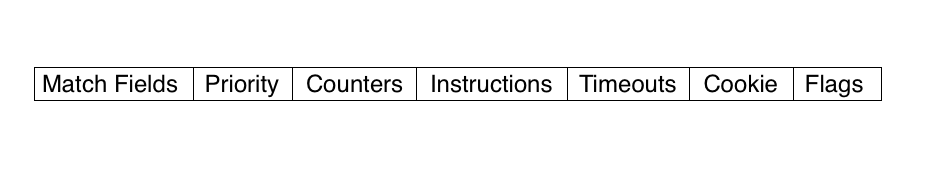
\includegraphics[width=1\textwidth]{figures/columns_of_flow_entry.png}
\end{center}
\caption{Columns of a flow entry. \sout{{\color{red} bad quality!!}}}
\label{FE_Col}
\end{figure}

\section{Topology discovery services}
\label{Topology discovery services}
To realize centralized control and high programmability, controllers need to maintain the visibility of the whole network. Therefore, topology discovery services play an important role in SDN. These services try to achieve automatic adjustment when the topology is altered, resulting in reducing manual effort significantly when it comes to network managing. The topology system includes three parts: switch discovery, host tracking and internal link.

\subsection{Switch discovery service and Host tracking service}
Switch discovery is rather simple. When a switch try to initiate a connection with controller, the OpenFlow channel will be established, and the information of the switch will be sent to the controller and stored for future usage. 

A controller maintains Host Profiles to keep track of the host location. When a Packet-Miss happens, a Packet\_In message will be sent to the controller along with the packet's information and the controller will look up the Host Profiles it maintains. If the Host Profile of the host cannot be found, controller will assume a new host join the network and add the information of the host. But if there is a conflict between the Host Profile and the Packet\_In message, the controller treats this as a host migration and update the location information of the Host Profile.

\subsection{Link discovery service}
\label{Link discovery service}
When we refer to Link discovery, we mean the procedure of discovering the link between switches. Since there has not been a standard for the link discovery in the OpenFlow controller, we will use the term \textit{OpenFLow Discovery Protocol} (OFDP) when mentioning it. Currently, although there are be some minor differences in detail, all the main stream controllers support OFDP.

OFDP leverages the Link Layer Discovery Protocol (LLDP) with subtle modification to perform topology discovery in an OpenFlow network. LLDP is originally implemented by Ethernet switch to exchange its identity and capabilities with a adjacent layer 2 peers. In legacy network, LLDP packets are sent regularly via each port of switches \cite{LLDP_WS}. The information learned from LLDP packets sent by neighbor is stored by all the switches and the packets will not be forwarded after a single hop. Figure~\ref{LLDP_frame} shows the structure of LLDP Ethernet frame structure. Each LLDP Data Unit contains a sequence of type-length-value (TLV). 

However, OFDP operates quite differently. The topology information is kept by the controller instead of OpenFlow switch, and an OpenFlow switch will do nothing more than forward the LLDP packet. The simplified process is shown in Figure~\ref{OFDP}. All switches have a pre-installed rule in their flow table, sending any LLDP packet received from any port, except the controller port, back to controller via Packet\_In. Initially, controller creates an individual LLDP packet for each port on every switches via Packet\_Out message. After receiving LLDP packet from controller, S1 sends it out on Port 1 and received by S2 on Port 3. With the pre-installed forwarding rule, switch S2 forwards the received LLDP packet to the controller via a Packet\_In message. This Packet\_In message contains meta-data such as the ID of the switch and the ingress port via which the packet was received. Thus, the controller can now infer that there exists a link between Port 1 of S1 and Port 3 of S2, and this information will be added to controller's topology database. After running this process through all ports on all the switches, controller is able to obtain all link between switches in the network. The entire discovery process is performed periodically with a typical default interval size of 5 seconds \cite{PPTI14}. 

\begin{figure}[H]
\begin{center} 
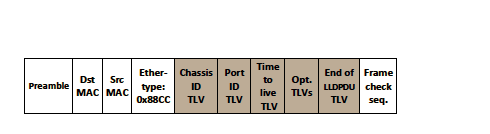
\includegraphics[width=1\textwidth]{figures/LLDP_packet_format.png}
\end{center}
\caption{LLDP packet frame structure. \cite{LLDP_WS}}
\label{LLDP_frame}
\end{figure}

\begin{figure}[H]
\begin{center} 
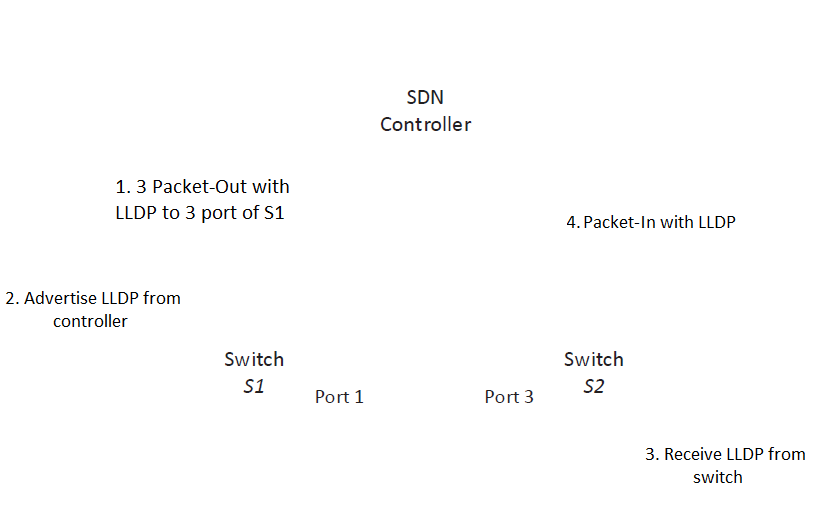
\includegraphics[width=1\textwidth]{figures/OFDP_procedure.png}
\end{center}
\caption{A illustration of OFDP procedure}
\label{OFDP}
\end{figure}

\section{SDN security}
\label{SDN security}
As SDN brings fascinating development and introduces new factors to network technology, there are a lot more vectors for us to concern about. Figure~\ref{SND_threat_overview} is a whole picture of attacks we discuss and where they might take place inside SDN, and Table~\ref{table:sdn_threats} contains further description of these threats. In this chapter, we will talk about SDN security-related issues. We will focus on some of them and discuss about the attack scenarios, possible consequences and countermeasures. 

\begin{figure}[H]
\begin{center} 
\includegraphics[width=1\textwidth]{figures/SDN_threat_overview.png}
\end{center}
\caption{SDN threat overview.}
\label{SND_threat_overview}
\end{figure}

\begin{table}[H]
\centering
\caption{Detail of each attack.}
\begin{tabular}{|l|p{4cm}|p{3.2cm}|p{5cm}|}
\hline ID & Threat name	& Location & Consequences \\
\hline
\hline 1 & System Vulnerability & all devices & Device compromised\\
\hline 2 & Administrative Interface Compromised & all administrative interfaces & Device compromised \\
\hline 3 & Application Vulnerability & SDN application & Malicious command to controller \\
\hline 4 & Host Hijacking & host & Attacker receives target host's traffic \\
\hline 5 & Link Fabrication & link between switch & Add non-existing link to controller's view \\
\hline 6 & Flow Entry Modification & switch & Unwanted packet redirection or drop \\
\hline 7 & Malicious Packet Controller DOS  & host, switch & DOS to controller \\
\hline 8 & Control-channel Hijacking & switch & Manipulate control traffic \\
\hline 
\end{tabular}
\label{table:sdn_threats}
\end{table}

\subsection{General security}
There are quite a few devices in SDN network, such as controllers, switches and hosts. All these devices possibly contain system vulnerabilities like Heartbleeding, Poodle and Shellshock \cite{HB,POODLE,SHELLSHOCK} found in recent years. Moreover, one might be able to gain unauthorized access to the network physically or virtually, by using trivial methods like brute forcing the administrative interface or a physical break in. To deal with these kind of threats, all the best practices for hardening servers are applicable. Autonomic trust management technique should be used to harden these components in the network \cite{YZP11}. Also, Diego et al. propose replication, dynamic device association and self-healing concepts in their work to reinforce the security \cite{KDFRV13}. As to the administrative interface, organizations should implement Role-Based Access Control (RBAC) policies and event logging \cite{FFR09}. With all these methods, the damage should be reduced if controller compromise should happen.

\subsection{Controller and control channel attack}
Controllers are in charge of the SDN network. Therefore, it is known as the most severe threat in SDN if a controller is taken over by an attacker. By manipulating the flows, one may cause Deny Of Service (DOS) between the desired connections or Man In The Middle (MITM) with spoofed Southbound API message to redirect flow to host they have access. Besides, all the sensitive information including information of devices, network topology and all the cryptographic keys, which reside in controller, will fall into attacker's hand, resulting in damage expansion. It is also hard to detect such a threat, since with what one can do with a controller, it is possible to avoid many intrusion detection methods. The possibilities of controller being compromised including malicious applications that send unwanted command through northbound API, vulnerabilities on controller or administrative stations etc.

With a compromised switch, one may also reconfigure it to use an attacker-controlled controller than the one it should. This type of attack is called Control-channel hijacking attack. By manipulating the control traffic, an attacker is able to spoof messages to the target controller. An attacker can also perform a DOS to the controller by deliberately crafting malicious packets for controller to process slowly with a switch or host. Nevertheless, this kind of attack depends on the design and implementation of the controller heavily \cite{AAS14}.

Phillip et al introduced FortNox, the security policy enforcement kernel, as a countermeasure to malicious applications. It implements a rule detection engine and role-based authentication to mediate all OpenFlow rule insertion requests \cite{PSYFTG12}. As to securing the control channel, using out-of-band network for control traffic can reduce the chance of undesired control channel manipulation. Also, one should always use cryptographic methods such as SSL/TLS to secure the channels. Even so, it is not enough. Vulnerabilities of SSL/TLS have been proposed and proven \cite{HRKC12}. Kreutz et al. propose the concept of dynamic trust model and replication to maintain a trustful relationship among the connections between controller and design a secure and dependable control platform to enforce security \cite{KDFRV13}. 

\subsection{Topology poisoning attacks}
So far, the topology poisoning attacks have been discussed in many papers. The main idea of this type of attack is to trick controller into believing the existence of a non-existing link to host or switch by exploiting traits of topology management service. One can initiate such type of attack with either a switch or a host.

In Host Location Hijacking Attack, attacker exploits the trait of Host Tracking Service. The attacker impersonates a target host by sending spoofed packet with the host's information with PACKET\_IN, and the controller will think that the target host has moved to a new location. But the truth is, the traffic of the target host is now redirected to the attacker's host \cite{HXWG15}. Another type of host-initiated attack is called Link Fabrication Attack. The attack is caused by the fact that OpenFlow controllers accept LLDP from all switch ports, even if it is connected to a host. After an attacker receives LLDP packet with a host, he can modify specific contents like DPID or port number of LLDP packets to launch a LLDP packet injection attack. To deal with these two types of host-initiated attack, Hong et al. present TopoGuard, a new security extension to OpenFlow controller. They verify the legitimacy of Host Migration by further inspecting sign of host migration, and manage port property in order to avoid any host residing inside the LLDP propagation \cite{HXWG15}.

However, LLDP packets are passed around with the aid of switches. The Link Fabrication Attack can also initiate by compromised switches, which is not included in the scenario of TopoGuard. Bui gives three different attack scenarios of Link Fabrication Attack with compromised switches, which are two-switch tunnel attack extended two-switch tunnel attack and single-switch attack, and evaluates their consequence under different routing algorithms and network topologies \cite{TTB15}. This attack is caused by the lack of authentication of LLDP. However, simply adding authenticator inside LLDP packet will not help against LLDP relay attack \cite{HXWG15}. Alharbi et al. implement HMAC based mechanism with a little modification to static secret key, which is able to detect the injection of any fabricated LLDP packets, with only an acceptable of amount of overhead added \cite{ATPP15}.

Besides link fabrication attacks, attackers can also modify the flow entries inside the flow tables of the compromised switch to perform MITM, eavesdropping or DOS attack \cite{AAS14}. The detection method proposed in \cite{CKGL15} is able to detect whether a switch is forwarding the packets in an unexpected way. After selecting a flow entry as the detecting target, they install new entry on its neighbors. With the match field selected by their algorithm, they are able to let every packet that matches the new flow entry matches the target flow entry. A packet containing the match field of the new flow entry will be sent from Packet\_Out to a neighbor of the target switch, forwarded to the target switch, and should be sent back to the controller. Finally, they will check if the packet comes back to the controller as expected and remain unchanged. However, this method will take a longer time to run if we want to scan through lots of flow entries. Pre-detection method to narrow down the potential target is needed.
